\documentclass[11pt,a4paper]{article}
\usepackage[utf8]{inputenc}
\usepackage[T1]{fontenc}
\usepackage[margin=1in]{geometry}
\usepackage{graphicx}
\usepackage{hyperref}
\usepackage{xcolor}
\usepackage{float}
\usepackage{listings}
\usepackage{upquote}
\usepackage{tcolorbox}
\tcbuselibrary{skins}

\lstset{
    basicstyle=\ttfamily\small,
    breaklines=true,
    breakatwhitespace=false,
    frame=single,
    numbers=left,
    numberstyle=\tiny,
    backgroundcolor=\color{gray!10},
    keywordstyle=\color{blue},
    commentstyle=\color{green!50!black},
    stringstyle=\color{red},
    showstringspaces=false
}

\newtcolorbox{notebox}{colback=blue!5,colframe=blue!40!black,title=Note,fonttitle=\bfseries}

\title{\textbf{Practice 4 -- Half-Term Challenge: Grabbing an Object}}
\author{
    Robotics and Cyber-Physical Systems \\
    School of Sciences and Engineering \\
    Tecnol\'ogico de Monterrey
}
\date{}

\begin{document}

\maketitle

\section*{Introduction}

In this challenge, you will combine perception, coordinate transforms, and
robot control to locate and pick up a red object. We will begin by exploring
how an object detected by a camera is located relative to the robot.

\subsection*{Before You Begin}

Open a terminal in the repository and update your copy:

\begin{lstlisting}[language=bash]
git pull
uv sync
\end{lstlisting}

Make sure a red object is visible before starting the exercise.

\section*{Part 1 -- Explore Object Localization}

\subsection*{Objective}

Run the existing red-object plotter to build an intuition for camera
transforms and object localization:

\begin{lstlisting}[language=bash]
uv run examples/plot_red_object.py
\end{lstlisting}

The camera window marks the detected object and displays its estimated
coordinates in metres. The 3D window plots the camera and object relative to
the robot base, where $+x$ is forward, $+y$ is left, and $+z$ is upward.

\begin{itemize}
    \item Pan and tilt the head. The plotted camera should move while the
          object's base-frame position remains approximately stable.
    \item Move the robot or the red object and observe how the reported
          coordinates change.
    \item Press \texttt{H} to switch between head and wrist controls. Use
          \texttt{I}, \texttt{J}, \texttt{K}, and \texttt{L} to move them.
\end{itemize}

To compare both cameras, change the selected camera and run the script again:

\begin{lstlisting}[language=Python]
CAMERA = WRIST_CAMERA
\end{lstlisting}

\begin{figure}[H]
    \centering
    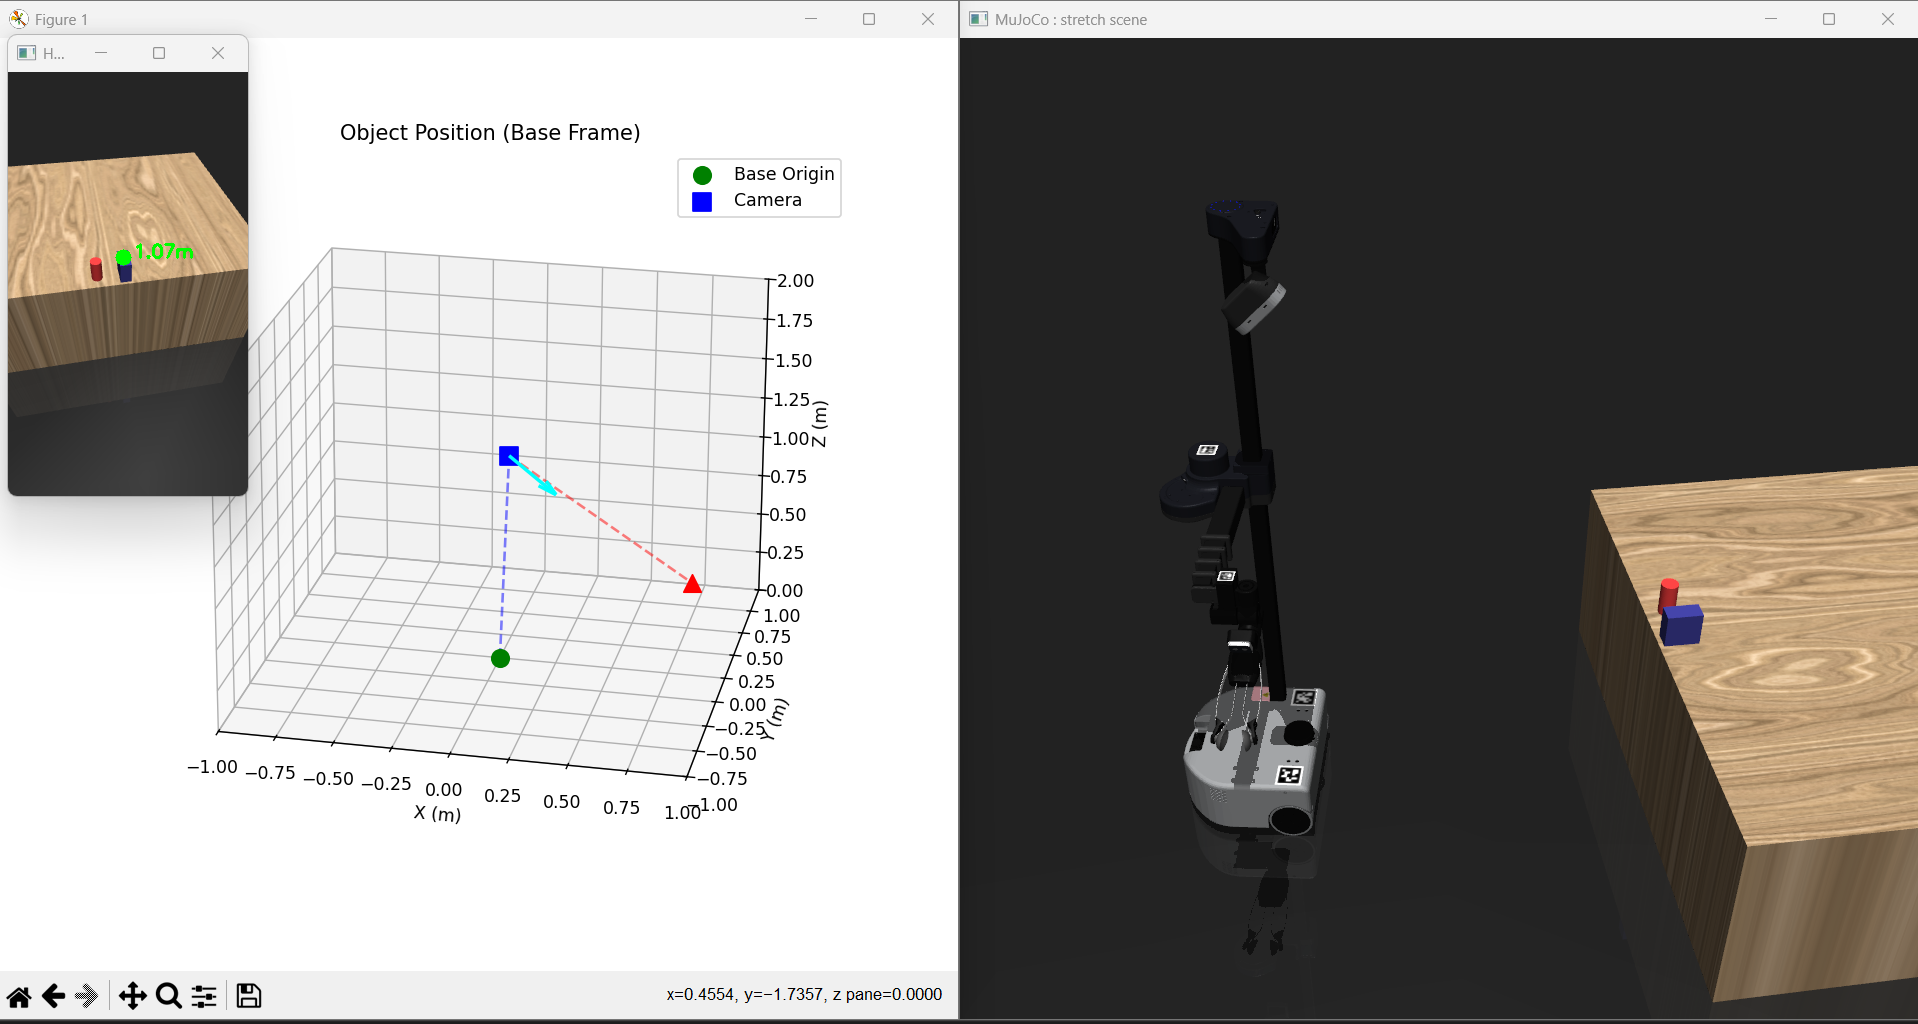
\includegraphics[width=0.85\textwidth]{p4_1_object_detected_and_plotter.png}
    \caption{Camera detection and 3D visualization of an object's position relative to the robot.}
    \label{fig:p4_object_plotter}
\end{figure}

\begin{notebox}
Small variations are expected from image detection and depth noise. When only
the camera moves, the estimated object should still remain approximately fixed
relative to the robot base.
\end{notebox}

\newpage

\section*{Part A -- Navigate Toward the Object}

In this part, you will build \texttt{p4a\_navigate.py} one behavior at a time.
Run the program after adding each command function before continuing to the
next one.

\subsection*{1. Copy the Boilerplate}

Create the new script from the teleoperation boilerplate:

\begin{lstlisting}[language=bash]
cp examples/teleop_boilerplate.py p4a_navigate.py
\end{lstlisting}

\subsection*{2. Add the Setup}

Replace the imports at the top of the new script with:

\begin{lstlisting}[language=Python]
import math

import cv2
import numpy as np

from stretch_tools import (
    HEAD_CAMERA,
    NormVelController,
    RobotTransforms,
    StateController,
    TeleopProvider,
    close_cameras,
)

try:
    import stretch_body.robot as robot
except ImportError:
    import stretch_mujoco_api.robot as robot
\end{lstlisting}

Add the controller constants below the imports:

\begin{lstlisting}[language=Python]
KP_HEAD = 0.5
KP_ROTATION = 1.0
KP_DISTANCE = 5.0
TARGET_DISTANCE = 0.6
NAVIGATION_MAX_DISTANCE = 3.0
FLANK_ANGLE = -math.pi / 2
FLANK_TOLERANCE = math.radians(5)
LIFT_HEIGHT_OFFSET = 0.0
SCAN_SPEED = -0.2
\end{lstlisting}

Copy these perception functions above \texttt{main()}:

\begin{lstlisting}[language=Python]
def detect_object(frame, depth_frame=None,
                  max_distance=None, camera_info=None):
    hsv = cv2.cvtColor(frame, cv2.COLOR_BGR2HSV)
    mask = cv2.inRange(
        hsv, np.array([0, 100, 100]),
        np.array([10, 255, 255])
    )
    mask |= cv2.inRange(
        hsv, np.array([170, 100, 100]),
        np.array([179, 255, 255])
    )
    contours, _ = cv2.findContours(
        mask, cv2.RETR_EXTERNAL, cv2.CHAIN_APPROX_SIMPLE
    )

    for contour in sorted(contours,
                          key=cv2.contourArea,
                          reverse=True):
        if cv2.contourArea(contour) <= 100:
            break
        moments = cv2.moments(contour)
        if not moments["m00"]:
            continue

        center = (
            int(moments["m10"] / moments["m00"]),
            int(moments["m01"] / moments["m00"]),
        )
        if depth_frame is not None and max_distance is not None:
            distance = camera_info.get_depth(center, depth_frame)
            if distance is None or distance > max_distance:
                continue
        return center

    return None


def locate_object(center, depth_frame, camera_info, camera_T):
    depth = camera_info.get_depth(center, depth_frame)
    if depth is None:
        return None

    x, y = camera_info.pixel_to_normalized(center)
    object_T = np.eye(4)
    object_T[:3, 3] = [x * depth, y * depth, depth]
    return camera_T @ object_T
\end{lstlisting}

Inside \texttt{main()}, replace the controller setup after robot startup with:

\begin{lstlisting}[language=Python]
controller = NormVelController(stretch, safe_base_mode=True)
teleop = TeleopProvider(robot=stretch)
transforms = RobotTransforms(stretch)

arm_stow = StateController(
    stretch,
    {
        "arm_out": 0.0,
        "wrist_pitch_up": -0.625,
        "wrist_roll_counterclockwise": 0.0,
        "wrist_yaw_counterclockwise": 2.994,
        "gripper_open": 1.0,
    },
)
lift_controller = StateController(stretch, {"lift_up": 0.3})
scanning_position = StateController(
    stretch,
    {
        "head_pan_counterclockwise": 0.0,
        "head_tilt_up": math.radians(-30),
    },
)

command = None
head_rgb, head_depth = None, None
head_center = None
object_T = None
within_distance = False
stowed = False
\end{lstlisting}

The variables are declared before the loop so the nested command functions
can use the latest camera data and command dictionary.

Use this camera and control structure inside the loop:

\begin{lstlisting}[language=Python]
command = {}
command.update(arm_stow.get_command())

success, head_rgb, head_depth = HEAD_CAMERA.get_frames()
if not success:
    return

head_center = detect_object(
    head_rgb, head_depth, NAVIGATION_MAX_DISTANCE, HEAD_CAMERA
)
stowed = arm_stow.is_at_goal()

if head_center is not None:
    cv2.circle(head_rgb, head_center, 5, (0, 255, 0), -1)

cv2.imshow("Head RGB", head_rgb)

command.update(lift_controller.get_command())
command = teleop.get_manual_override(command)
controller.set_command(command)

if cv2.waitKey(1) & 0xFF == ord("q"):
    break
\end{lstlisting}

Finally, add camera cleanup to the \texttt{finally} block:

\begin{lstlisting}[language=Python]
close_cameras()
cv2.destroyAllWindows()
stretch.stop()
\end{lstlisting}

Run the setup once before adding autonomous movement:

\begin{lstlisting}[language=bash]
uv run p4a_navigate.py
\end{lstlisting}

\subsection*{3. Add Scanning}

Add this nested function before the \texttt{try} block in \texttt{main()}:

\begin{lstlisting}[language=Python]
def scan():
    command.update(scanning_position.get_command())
    command["base_counterclockwise"] = SCAN_SPEED
\end{lstlisting}

Replace the simple detection check inside the loop with:

\begin{lstlisting}[language=Python]
if head_center is None:
    if stowed:
        scan()
else:
    cv2.circle(head_rgb, head_center, 5, (0, 255, 0), -1)
\end{lstlisting}

Run the script. The robot should first reach its safe stowed pose, then rotate
while holding the head in the scanning position. Stop the program before
continuing.

\subsection*{4. Add Head Tracking}

Add the second nested function after \texttt{scan()}:

\begin{lstlisting}[language=Python]
def track_with_head():
    x, y = head_center
    height, width = head_rgb.shape[:2]
    horizontal_error = (x - width / 2) / (width / 2)
    vertical_error = (y - height / 2) / (height / 2)
    command["head_pan_counterclockwise"] = \
        -KP_HEAD * horizontal_error
    command["head_tilt_up"] = -KP_HEAD * vertical_error
\end{lstlisting}

Call it when the object is visible:

\begin{lstlisting}[language=Python]
if head_center is None:
    if stowed:
        scan()
else:
    track_with_head()
    cv2.circle(head_rgb, head_center, 5, (0, 255, 0), -1)
\end{lstlisting}

Run the script again. When the red object enters the image, the base should
stop scanning and the head should keep the object centered.

\subsection*{5. Add Navigation}

Add the final nested command function:

\begin{lstlisting}[language=Python]
def navigate_to_object():
    nonlocal within_distance

    object_x, object_y, object_z = object_T[:3, 3]
    distance = math.hypot(object_x, object_y)
    facing_error = math.atan2(object_y, object_x)

    if within_distance:
        within_distance = 0.5 <= distance <= 0.7
    else:
        within_distance = 0.55 <= distance <= 0.65

    if within_distance:
        flank_error = math.atan2(
            math.sin(facing_error - FLANK_ANGLE),
            math.cos(facing_error - FLANK_ANGLE),
        )
        command["base_counterclockwise"] = \
            KP_ROTATION * flank_error

        if abs(flank_error) <= FLANK_TOLERANCE:
            lift_controller.desired_state["lift_up"] = \
                object_z - LIFT_HEIGHT_OFFSET
    else:
        alignment = max(
            0.0,
            1.0 - abs(facing_error) / (math.pi / 2),
        )
        command["base_counterclockwise"] = \
            KP_ROTATION * facing_error
        command["base_forward"] = alignment * KP_DISTANCE * (
            distance - TARGET_DISTANCE
        )
\end{lstlisting}

After \texttt{track\_with\_head()}, locate the object and call the navigation
function:

\begin{lstlisting}[language=Python]
else:
    track_with_head()
    object_T = locate_object(
        head_center,
        head_depth,
        HEAD_CAMERA,
        transforms.get_cam_T(HEAD_CAMERA),
    )
    if object_T is not None and stowed:
        navigate_to_object()
    cv2.circle(head_rgb, head_center, 5, (0, 255, 0), -1)
\end{lstlisting}

Run the completed program. The robot should scan until it sees the red object,
track it with the head, face and approach it, then rotate into a flank pose at
approximately $0.6$\,m. Forward movement is reduced while the robot is poorly
aligned, and distance hysteresis prevents rapid switching near the target.

\newpage

\section*{Part B -- Grab the Object}

Part A leaves the robot beside the object with the lift at the correct height.
You will now switch to the wrist camera, align the gripper, extend the arm,
close the gripper, and raise the object. Continue testing after every new
function.

\subsection*{1. Copy Part A}

Keep the completed navigation script and create Part B from it:

\begin{lstlisting}[language=bash]
cp p4a_navigate.py p4b_grab.py
\end{lstlisting}

Add \texttt{time} and \texttt{WRIST\_CAMERA} to the imports:

\begin{lstlisting}[language=Python]
import math
import time

import cv2
import numpy as np

from stretch_tools import (
    HEAD_CAMERA,
    WRIST_CAMERA,
    NormVelController,
    RobotTransforms,
    StateController,
    TeleopProvider,
    close_cameras,
)
\end{lstlisting}

Add the wrist and gripper constants:

\begin{lstlisting}[language=Python]
KP_WRIST = 0.5
KP_ARM = 5.0
TARGET_WRIST_DISTANCE = 0.15
WRIST_CENTER_TOLERANCE = 0.75
ARM_DISTANCE_TOLERANCE = 0.025
GRAB_POSITION_SETTLE_TIME = 0.5
LIFT_TOP = 1.1
WRIST_X_OFFSET = 25
WRIST_Y_OFFSET = 75
\end{lstlisting}

\subsection*{2. Add the Grab Setup}

After \texttt{scanning\_position}, create the wrist and gripper controllers:

\begin{lstlisting}[language=Python]
deploy_wrist = StateController(
    stretch,
    {
        "wrist_pitch_up": 0.0,
        "wrist_roll_counterclockwise": 0.0,
        "wrist_yaw_counterclockwise": 0.0,
    },
)
gripper_open_controller = StateController(
    stretch, {"gripper_open": 130.0}
)
gripper_close_controller = StateController(
    stretch, {"gripper_open": -25.0}
)
\end{lstlisting}

Add the wrist data and grab state below the Part A variables:

\begin{lstlisting}[language=Python]
wrist_rgb, wrist_depth = None, None
wrist_center = None

gripper_ready = False
gripper_closing = False
grab_position_started = None
ready_to_close = False
grabbed = False
phase = "navigate"
\end{lstlisting}

\subsection*{3. Add the Phase Transition}

The Part A logic becomes the navigation phase. Change the beginning of the
loop from:

\begin{lstlisting}[language=Python]
command = {}
command.update(arm_stow.get_command())
\end{lstlisting}

to:

\begin{lstlisting}[language=Python]
command = {}

if phase == "navigate":
    command.update(arm_stow.get_command())
    # Indent the remaining Part A camera and navigation logic here.
else:
    # Grab logic will be added in the following steps.
    pass
\end{lstlisting}

The common commands at the bottom of the loop remain outside the phase check:

\begin{lstlisting}[language=Python]
command.update(lift_controller.get_command())
command = teleop.get_manual_override(command)
controller.set_command(command)
\end{lstlisting}

Update the first line of \texttt{navigate\_to\_object()} so it can change the
phase:

\begin{lstlisting}[language=Python]
nonlocal within_distance, phase
\end{lstlisting}

Then replace the lift update inside its flank-aligned condition with:

\begin{lstlisting}[language=Python]
lift_controller.desired_state["lift_up"] = \
    object_z - LIFT_HEIGHT_OFFSET

if lift_controller.is_at_goal():
    phase = "grab"
    print(f"\nPhase: {phase}")
\end{lstlisting}

For the first test, place this temporary grab block in the loop's
\texttt{else} branch:

\begin{lstlisting}[language=Python]
command["arm_out"] = 0.0
command.update(deploy_wrist.get_command())
command.update(gripper_open_controller.get_command())

success, wrist_rgb, wrist_depth = WRIST_CAMERA.get_frames()
if success:
    wrist_center = detect_object(wrist_rgb)
    cv2.imshow("Wrist RGB", wrist_rgb)
    depth_display = cv2.normalize(
        wrist_depth, None, 0, 255,
        cv2.NORM_MINMAX, cv2.CV_8U
    )
    cv2.imshow("Wrist Depth", depth_display)
\end{lstlisting}

Run the program. It should navigate into the flank pose, raise the lift, switch
to the wrist camera, deploy the wrist, and open the gripper.

\subsection*{4. Center the Object with the Wrist}

Add this nested function after the navigation functions:

\begin{lstlisting}[language=Python]
def center_object_with_wrist():
    x, y = wrist_center
    height, width = wrist_rgb.shape[:2]
    horizontal_error = \
        (x - width / 2 - WRIST_X_OFFSET) / (width / 2)
    vertical_error = \
        (y - height / 2 - WRIST_Y_OFFSET) / (height / 2)

    command["wrist_yaw_counterclockwise"] = \
        -KP_WRIST * horizontal_error
    command["wrist_pitch_up"] = \
        -KP_WRIST * vertical_error

    cv2.circle(wrist_rgb, wrist_center, 5, (0, 255, 0), -1)
    return horizontal_error, vertical_error
\end{lstlisting}

Call it after detecting the object in the grab branch:

\begin{lstlisting}[language=Python]
if wrist_center and not grabbed:
    horizontal_error, vertical_error = \
        center_object_with_wrist()
\end{lstlisting}

Run the script again. The wrist pitch and yaw should keep the green point near
the desired grasping location in the image.

\subsection*{5. Reach for the Object}

Add the arm controller:

\begin{lstlisting}[language=Python]
def reach_for_object(horizontal_error, vertical_error):
    nonlocal ready_to_close

    if gripper_ready:
        distance = WRIST_CAMERA.get_depth(
            wrist_center,
            wrist_depth,
            sample_radius=15,
        )
        if distance is not None:
            center_error = math.hypot(
                horizontal_error, vertical_error
            )
            authority = max(0.0, 1.0 - center_error)
            command["arm_out"] = authority * KP_ARM * (
                distance - TARGET_WRIST_DISTANCE
            )
            ready_to_close = (
                center_error <= WRIST_CENTER_TOLERANCE
                and abs(distance - TARGET_WRIST_DISTANCE)
                <= ARM_DISTANCE_TOLERANCE
            )
\end{lstlisting}

At the start of the grab branch, reset the temporary condition and latch the
gripper-open state:

\begin{lstlisting}[language=Python]
ready_to_close = False
command["arm_out"] = 0.0
command.update(deploy_wrist.get_command())

if gripper_open_controller.is_at_goal():
    gripper_ready = True
\end{lstlisting}

Call the reach controller immediately after wrist centering:

\begin{lstlisting}[language=Python]
if wrist_center and not grabbed:
    horizontal_error, vertical_error = \
        center_object_with_wrist()
    reach_for_object(horizontal_error, vertical_error)
\end{lstlisting}

Keep applying \texttt{gripper\_open\_controller.get\_command()} for now and
run the program. Once the gripper is open, the arm should extend toward
$0.15$\,m. The alignment-based authority reduces arm movement when the object
is far from its desired image position.

\subsection*{6. Close and Lift}

Add the final nested function:

\begin{lstlisting}[language=Python]
def update_gripper():
    nonlocal grab_position_started, gripper_closing, grabbed

    if not gripper_closing:
        if ready_to_close:
            if grab_position_started is None:
                grab_position_started = time.monotonic()
            elif (
                time.monotonic() - grab_position_started
                >= GRAB_POSITION_SETTLE_TIME
            ):
                gripper_closing = True
                print("\nGrabbing position reached")
        else:
            grab_position_started = None

    if gripper_closing:
        command.update(gripper_close_controller.get_command())
    else:
        command.update(gripper_open_controller.get_command())

    if (
        gripper_closing
        and not grabbed
        and gripper_close_controller.is_at_goal()
    ):
        grabbed = True
        lift_controller.desired_state["lift_up"] = LIFT_TOP
        print("\nObject grabbed")

    if grabbed:
        command["arm_out"] = 0.0
        command["wrist_pitch_up"] = 0.0
        command["wrist_roll_counterclockwise"] = 0.0
        command["wrist_yaw_counterclockwise"] = 0.0
\end{lstlisting}

Remove the temporary direct gripper-open command from the grab branch. Call
the new function after processing the wrist frame:

\begin{lstlisting}[language=Python]
update_gripper()
\end{lstlisting}

The gripper closes only after the image and depth conditions remain satisfied
for half a second. Once the close controller settles, the visual servo stops
and the lift target changes to its upper position.

\subsection*{Expected Result}

Run the complete script:

\begin{lstlisting}[language=bash]
uv run p4b_grab.py
\end{lstlisting}

The robot should complete this sequence:

\begin{enumerate}
    \item Stow safely and scan for the red object.
    \item Track, approach, and present its flank at approximately $0.6$\,m.
    \item Raise the lift and deploy the wrist.
    \item Center the object with wrist pitch and yaw.
    \item Extend the arm until the object is approximately $0.15$\,m away.
    \item Close the gripper and raise the object.
\end{enumerate}

Keep the emergency stop accessible and clear the robot's complete motion area
before every test. Collision management must remain enabled.

\begin{figure}[H]
    \centering
    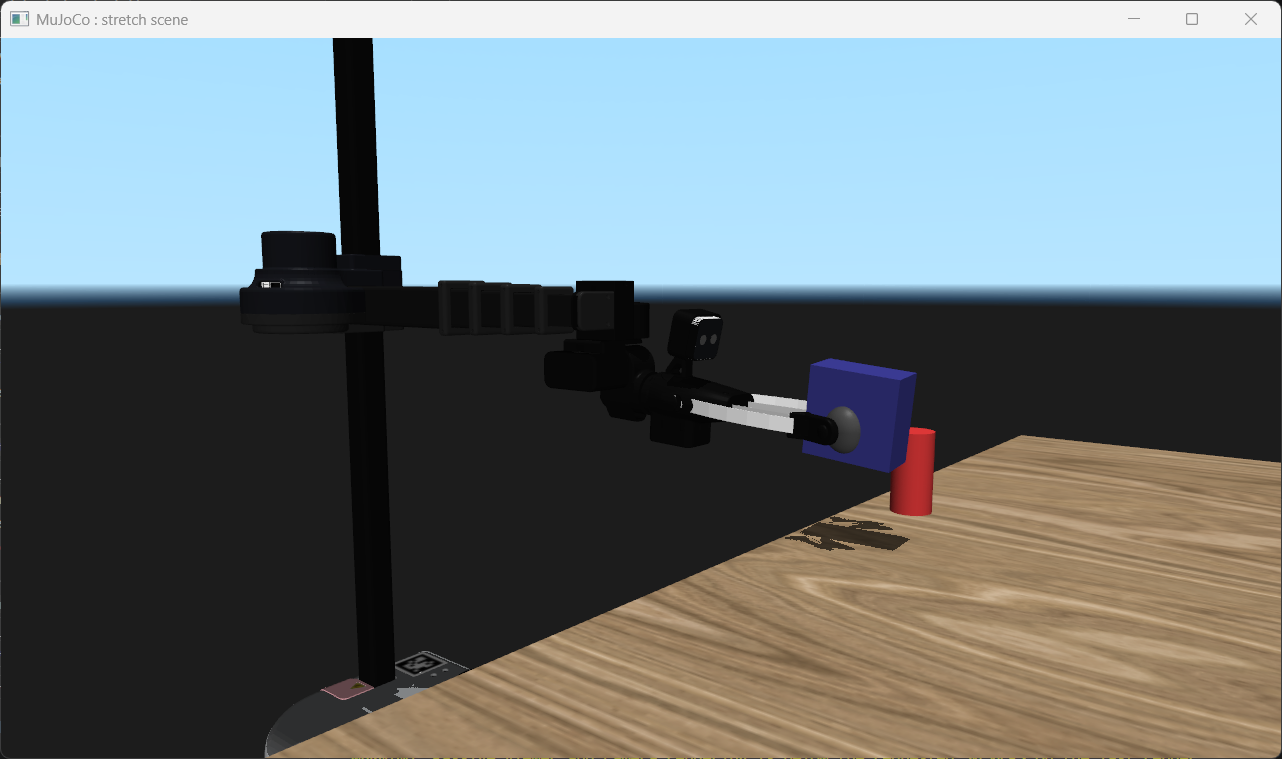
\includegraphics[width=0.85\textwidth]{p4_5_gripper_closed_object_lifted.png}
    \caption{The completed autonomous grab with the object secured and lifted.}
    \label{fig:p4_complete_grab}
\end{figure}

\newpage

\section*{Deliverable}

Submit a screen recording with voiceover showing \texttt{p4b\_grab.py}
completing the full sequence without manual assistance. The recording must
show the camera windows, terminal phase messages, and the robot's complete
motion from scanning through lifting the object.

Briefly explain how RGB detection, depth, \texttt{RobotTransforms},
proportional control, and the grab latches contribute to the final behavior.

\end{document}
